\documentclass[a4paper]{article}

%% Language and font encodings
\usepackage[english]{babel}
\usepackage[utf8x]{inputenc}
\usepackage[T1]{fontenc}

%% Sets page size and margins
\usepackage[a4paper,top=3cm,bottom=2cm,left=3cm,right=3cm,marginparwidth=1.75cm]{geometry}

%% Useful packages
\usepackage{amsmath}
\usepackage{graphicx}
\usepackage[colorinlistoftodos]{todonotes}
\usepackage[colorlinks=true, allcolors=blue]{hyperref}

\title{Analysis Note: \\
Measurement of $D^0$-meson production in Au+Au collisions at $\sqrt{s_{\rm NN}}$ = 200\,GeV}
\author{Xiaolong Chen, Xin Dong, Mustafa Mustafa, Guannan Xie, Yifei Zhang, Long Zhou}

\begin{document}
\maketitle

\begin{abstract}
Your abstract.
This is just a test

Heavy quarks nuclear modification factor ($R_{AA}$) has been proposed as an important measurement to study the flavor dependence of partons energy loss in the medium, and eventually to help in extracting the medium transport, drag and diffusion coefficients.

We report the first measurement of efficiency corrected spectrum for $D^0$ from HFT through the hadronic channels ($D^0(\bar{D^0}) \rightarrow K^{\mp}\pi^{\pm}$), the Nuclear Modification Factor ($R_{AA}$) of $D^0$ mesons in Au+Au collisions at $\sqrt{s_{NN}}$ = 200 GeV. The precision was much better compared to previous published one. The new $R_{AA}$ results show significant suppression at high $p_T$ which means the strong interaction between charm quark and the medium and loose energy. While the $D^0$ $R_{AA}$ shows quite similar trend as light hadrons.

\end{abstract}

\section{Introduction}

Heavy quarks nuclear modification factor ($R_{AA}$) has been proposed as an important measurement to study the flavor dependence of partons energy loss in the medium, and eventually to help in extracting the medium transport, drag and diffusion coefficients. There are lots of theoretical calculations for the energy losses for different flavor particles. Fig.~\ref{fig:raa_CUJE} shows the jet flavor tomography level crossing pattern of nuclear modification factors at middle rapidity of $\pi$, D, B, e from CUJT calculations for central Au + Au 200 GeV collisions. As clearly see the mass hierarchy of the different flavor energy loss.

\begin{figure}
\centering
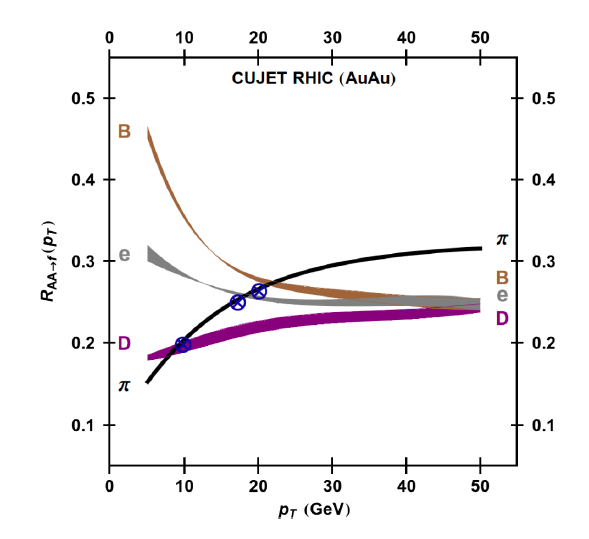
\includegraphics[width=0.5\textwidth]{fig/raa_CUJE.png}
\caption{Jet flavor tomography level crossing pattern of nuclear modification factors at middle rapidity of $\pi$, D, B, e calculations for central Au + Au 200 GeV collisions.}
\label{fig:raa_CUJE} 
\end{figure}

The hadronic channels allow to fully reconstruct the charmed hadrons and do not suffer from the complications in the semi-leptonic decays, however the measurement can be challenging due to large combinatorial backgrounds and lower branching ratios. One approach is to use the decay topology to reduce this background by distinguishing between tracks that come from the collision itself (primary vertex) and those from a secondary decay vertex. This requires the detectors must be able to resolve differences on the order of tens of microns. Heavy Flavor Tracker (HFT) is essence the right detector for this mission.

\section{\label{dataset}Datasets and Event Selection}

The dataset used in this analysis is P16id production of 2014 Au+Au 200 GeV data. This is the first year of physics running the new STAR HFT Detector. The analysis uses picoDst which is produced from MuDst.

The Minimum-Bias (MinBias) trigger is defined as a coincidence between the two VPDs, and an online collision vertex cut. Moreover, a pile-up protection at the trigger level was applied for the data taking. In this analysis, the MinBias trigger, denoted as ``vpdmb-5-p-nobsmd" and ``vpdmb-5-p-nobsmd-hlt", is used. The triggers used in this analysis are listed in Table.

\begin{table}[htp]
\centering
\caption{Triggers ID used in this analysis from run14}
\label{trigger}
	\begin{center}
	\begin{tabular}{l|l}
 \Xhline{1.6pt}
	Trigger ID	& description\\ \hline
	450050		& vpdmb-5-p-nobsmd-hlt\\ \hline
	450060		& vpdmb-5-p-nobsmd-hlt\\ \hline
	450005		& vpdmb-5-p-nobsmd\\ \hline
	450015		& vpdmb-5-p-nobsmd\\ \hline
	450025		& vpdmb-5-p-nobsmd\\ \hline
 \Xhline{1.6pt}
	\end{tabular}
	\end{center}
\end{table}

\subsection{Centrality Definition}



\section{$D^0$ Reconstruction}

\subsection{Topological Cut Optimization}

\section{$D^0$ Reconstruction}

\section{Efficiency Correction}
General idea.....

\subsection{TPC Tracking Efficiency}

\subsection{Data-driven fast Monte Carlo setup for HFT and Topological Cut Efficiency}

\subsection{Validation with Full GEANT+Hijing Simulation}

\subsection{PID Efficiency and Double Counting Correction}

The PID efficiency part includes the efficiency from $dE/dx$ or $n\sigma$ cut efficiency and the TOF matching+$1/\beta$ cut efficiency. The $dE/dx$ and $1/\beta$ calibration usually uses a specific set of tracks. The performance for identified particles that pass our analysis cut may not necessarily be exactly normal Gaussian distributions with means=0 and widths=1. It is desired to calibrate each individual distributions for identified particles for efficiency correction and mis-PID effect study.

For $n\sigma$ calibration, we followed the same method as described in Ref.~\cite{Xu:2008th} to calibrate high $p_{\rm T}$ pions and protons by selecting daughters from $K_{S}^0$ and $\Lambda$ decays.

\subsubsection{$dE/dx$ Calibration}



\subsection{Vertex Resolution Correction}

\subsection{Validation with Ks Spectra Measurement}

\begin{figure}
\centering
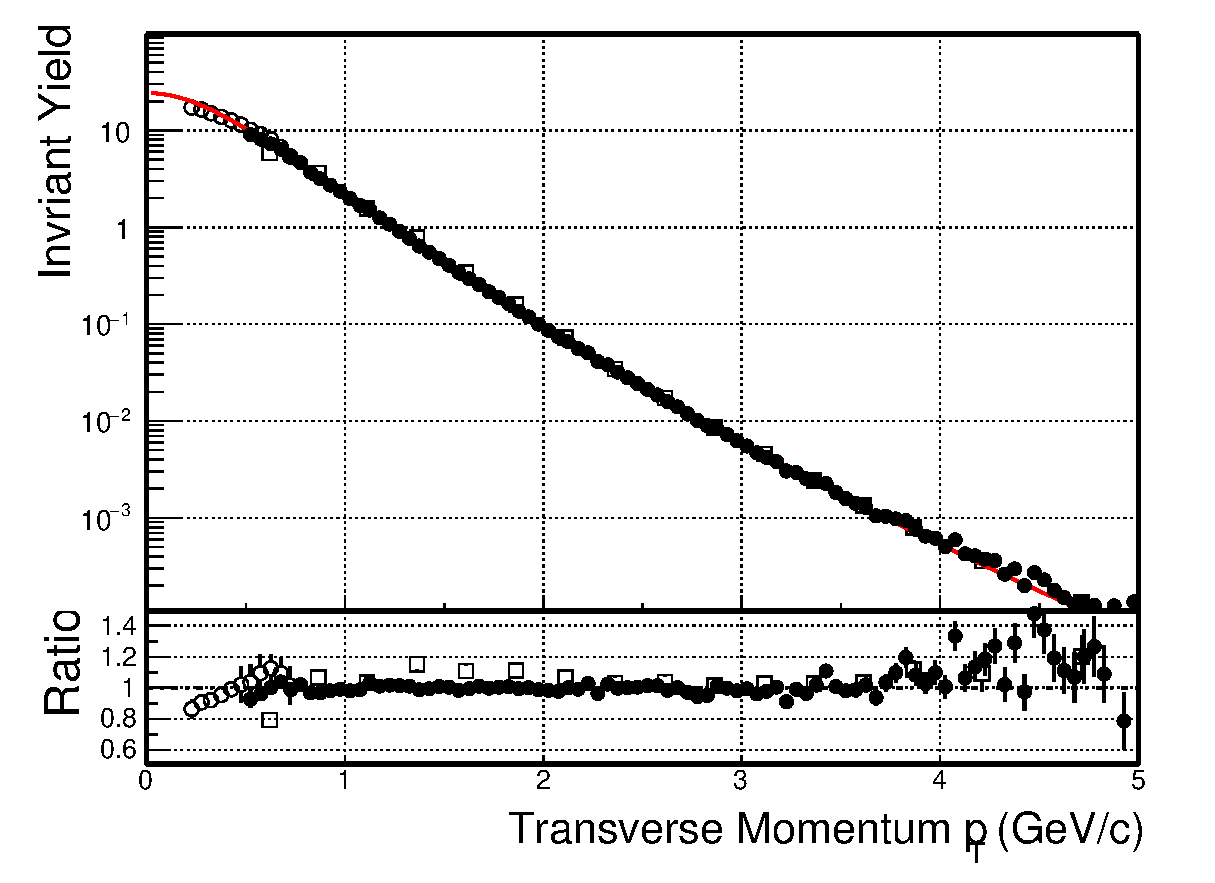
\includegraphics[width=0.7\textwidth]{fig/Ks_spectra_PtCut_0.eps}
\caption{\label{fig:Ks_spectra}Ks spectra.}
\end{figure}

\section{\label{results}Results}

\section{\label{Run1011}Re-analysis of Run10/11 data}

\subsection{Long and Yifei's re-analysis}

\subsection{Xiaolong's re-analysis}

\section{\label{Run14TPC}Run14 TPC analysis}

\bibliographystyle{alpha}
\bibliography{D0spectra_Note}

\end{document}
